\documentclass[../main/main.tex]{subfiles}
\graphicspath{{./figures/}}
\usepackage{pdfpages}

\makeatletter
\renewcommand{\@chapapp}{Travaux pratiques -- TP}
\makeatother

\toggletrue{student}
\HideSolutionstrue
\toggletrue{corrige}
% \renewcommand{\mycol}{black}
\renewcommand{\mycol}{gray}

\begin{document}
\setcounter{chapter}{12}

\chapter{\cswitch{Correction du TP}{\'Etude d'un filtre passe-bas du premier ordre}}

\begin{pycode}
import numpy as np
import cmath
R = 1e3           # Ohm
C = 0.1e-6        # Farad
wc = 1/(R*C)      # rad.s^-1
fc = wc/(2*np.pi) # Hz
def H(f):
    return (1/(1+1j*(f/fc)))
def G(f):
    return (20*np.log10(abs(H(f))))
def F(f):
    return (cmath.phase(H(f)))
def T(f):
    return F(f)/(2*np.pi*f)
# fmin = 1e2        # Hz
# fmax = 5e4        # Hz
# plist = np.array(
# [0, 0.05, 0.1, 0.12, 0.145, 0.2, 0.3, 0.4, 0.5, 0.6, 0.8, 0.9, 1]
# )
flist = [100, 300, 600,
				1000, 1200, 1600, 2000, 3000, 5000, 7000,
				10000, 20000, 30000, 40000, 50000]
\end{pycode}

\enonce{
	\begin{prgm}
		\begin{tcb}*(ror)"know"{Savoir}
			\begin{itemize}
				\item Décalage temporel/Déphasage à l'aide d'un oscilloscope numérique.
				\item Reconnaître une avance ou un retard.
			\end{itemize}
		\end{tcb}
		\begin{tcb}*(ror)"how"{Savoir-faire}
			\begin{itemize}
				\item Mettre en œuvre un dispositif expérimental illustrant l’utilité
				      des fonctions de transfert pour un système linéaire à un ou plusieurs
				      étages.
				\item Passer d'un décalage temporel à un déphasage et inversement.
				\item Agir sur un signal électrique à l'aide des fonctions simples
				      suivantes~: filtrage
			\end{itemize}
		\end{tcb}
	\end{prgm}
	\vspace{-10pt}
	\section{Objectifs}
	\begin{itemize}
		\item Apprendre à utiliser un dBmètre.
		\item Apprendre à déterminer rapidement une fréquence de coupure.
		\item Apprendre à mesurer un déphasage à l'oscilloscope.
		\item Apprendre à tracer un diagramme de \textsc{Bode} sur papier semi-log et
		      papier millimétré.
	\end{itemize}
}

\enonce{%
	\section{S'approprier}

	\subsection{Méthode pour mesurer un déphasage -- rappel de cours}

	Supposons $e(t) = E_{m} \cos(\w t)$ sur la voie $Y_1$ et $s(t) = S_{m} \cos (\w
		t + \f)$ sur la voie $Y_2$ de l'oscillogramme ci-contre.  Le déphasage $\f$
	entre deux signaux est un nombre appartenant à l'intervalle $\left]-\pi~;
		\pi\right]$. Il se mesure grâce à l'oscilloscope.
	\smallbreak
	\noindent
	\begin{minipage}[c]{.60\linewidth}
		\begin{enumerate}
			\item \xul{Déterminer la valeur absolue de $\Delta\f_{s/e}$}~: pour cela, il
			      faut placer les curseurs verticaux de manière à déterminer le
			      décalage temporel $\Delta t$, puis $\abs{\Delta\f_{s/e}} =
				      \w\Delta{t}$ (en rad).
			\item \xul{Ensuite déterminer le signe de $\Delta\f_{s/e}$}~:
			      pour cela, on cherche quelle courbe est en avance sur l'autre. Sur
			      l'oscillogramme ci-contre, $s$ est en retard sur $e$ puisqu'il s'annule
			      après $e$~: on en déduit $\Delta\f_{s/e} < 0$.
		\end{enumerate}
	\end{minipage}
	\hfill
	\begin{minipage}[c]{.40\linewidth}
		\begin{center}
			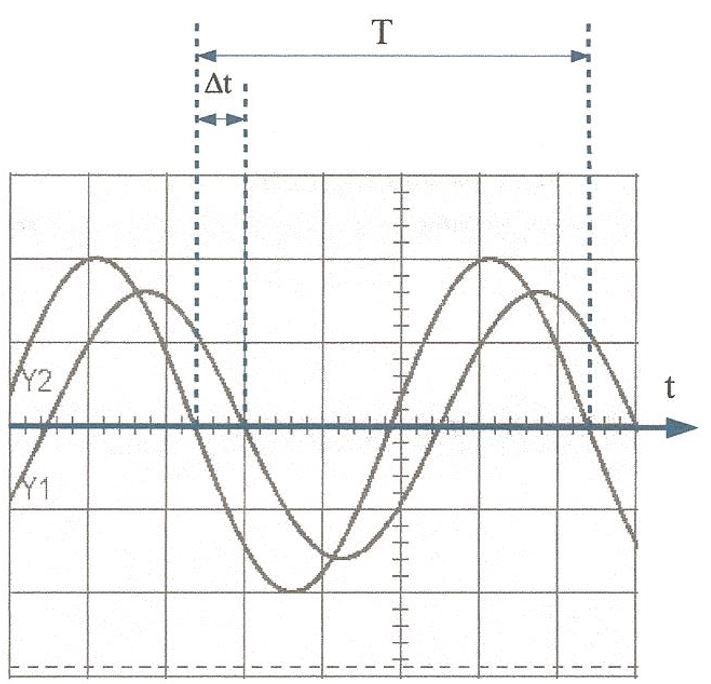
\includegraphics[width=\linewidth]{dephasage}
			\captionof{figure}{Déphasage}
			\label{fig:dephasage}
		\end{center}
	\end{minipage}

	\subsection{Méthode pour mesurer un gain en dB}

	Le gain se mesure grâce à un multimètre.
	\begin{tcb}(expe)<itc>{Mesure de gain}
		\begin{enumerate}
      \item Appuyez sur la fonction Volt alternatif (symbole
            \fbox{V$\sim$}), \textbf{puis} dBmètre (bouton \fbox{dB}) pour
            activer la fonction dBmètre~;
			\item Brancher le multimètre sur l'entrée $e(t)$ du montage~;
			\item Appuyer sur \fbox{\texttt{rel}} une ou deux fois jusqu'à ce que le
			      multimètre affiche 0~: on indique alors au multimètre que c'est cette
			      tension $e(t)$ qui sert de référence.
			\item Brancher ensuite le multimètre sur la sortie $s(t)$. Il affiche
			      directement le gain en dB.
		\end{enumerate}
		\begin{center}
			\begin{tcb}[cnt, bld, width=.8\linewidth](impo){Attention}
				Il faut refaire le zéro relatif pour chaque fréquence.
			\end{tcb}
		\end{center}
	\end{tcb}

	\subsection{Méthode pour tracer un diagramme de \textsc{Bode}}

	Pour tracer le diagramme de \textsc{Bode}, il est nécessaire pour chaque
	fréquence de déterminer~:
	\begin{enumerate}
		\item le déphasage $\Delta\f_{s/e}$ de $s(t)$ par rapport à $e(t)$~;
		\item Le gain en dB.
	\end{enumerate}
}

\setcounter{section}{2}
\section{Analyser}

\begin{minipage}{0.60\linewidth}
	Le montage étudié, schématisé ci-contre, est un circuit RC série alimenté
	par la tension $e(t) = E_{m} \cos(\w t)$. On pose $s(t) = S_{m} \cos (\w t +
		\f)$ la tension aux bornes du condensateur.
\end{minipage}
\hfill
\begin{minipage}{0.35\linewidth}
	\begin{center}
		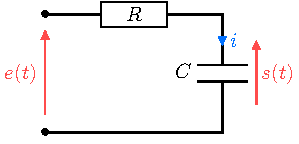
\includegraphics[width=\linewidth]{filtre_rc}
	\end{center}
\end{minipage}

\setlist[blocQR,1]{leftmargin=10pt, label=\clenumi}

\QR{%
	Établir l'expression de la fonction de transfert.
}{%
	Pont diviseur~:
	\begin{DispWithArrows*}
		\Su &= \frac{1/\jcw}{R + 1/\jcw}\Eu
		\CArrow{$\times \frac{\jcw}{\jcw}$}
		\\\Lra
		\Su &= \frac{1}{1+\jrcw}\Eu
		\Arrow{$\Hu = \Su/\Eu$}
		\\\Lra
		\Hu &= \frac{1}{1+\jrcw}
		\Arrow{$\w_c = \frac{1}{RC}$}
		\\\Lra
		\Hu &= \frac{1}{1+\jj \frac{\w}{\w_c}}
		\Arrow{$x = \frac{\w}{\w_c}$}
		\\\Lra
		\Aboxed{\Hu &= \frac{1}{1+\jx}}
	\end{DispWithArrows*}
}

\QR{%
	Déterminer le comportement asymptotique du filtre pour le gain et le
	déphasage.
}{%
	\begin{enumerate}
		\mitem
		\[
			\boxed{
				\Hu(x) \opto{}{x\to 0} \frac{1}{1 + 0} = 1
				\qet
				\Hu(x) \opto{}{x\to \infty} \frac{1}{\jx}
			}
		\]
		\vspace{-15pt}
		\item
		      \begin{itemize}
			      \item Pour le gain~:
			            \[
				            G\ind{dB}(x) \opto{}{x\to 0} 20 \log (1) = 0
				            \qet
				            G\ind{dB}(x) \opto{}{x\to\infty}
				            20 \log \abs{\frac{1}{\jx}} = -20 \log x
			            \]
			            %
			            Ainsi, à hautes fréquences, \textbf{le gain diminue de
				            \SI{20}{dB} par décade}~: si $\w$ est multiplié par 10, le
			            gain en décibel baisse de \SI{20}{dB} (i.e.\ l'amplitude est
			            divisée par 10).
			      \item Pour la phase~:
			            \[
				            \f(x) \opto{}{x\to 0} \arg*{1} = 0
				            \qet
				            \f(x) \opto{}{x\to \infty}
				            \arg*{\frac{1}{\jx}} = -\frac{\pi}{2}
			            \]
			            \vspace{-15pt}
		      \end{itemize}
	\end{enumerate}
}

\QR{%
	Déterminer l'expression de la fréquence de coupure $f_{c}$, puis la
	calculer pour $R=\SI{1,0}{k\ohm}$ et $C = \SI{0,10}{\micro F}$.
	\pyc{R = 1e3; C=0.1e-6; fc = 1/(R*C*2*3.1415)}
}{%
	On a trouvé
	\begin{gather*}
		\w_c = \frac{1}{RC} \Lra \boxed{f_c = \frac{1}{2\pi RC}}
		\qav
		\left\{
		\begin{array}{rcl}
			R & = & \SI{1.0}{k\ohm}
			\\
			C & = & \SI{0.10}{\micro F}
		\end{array}
		\right.\\
		\AN
		\xul{
			f_c = \py{fr'\SI{{{fc:.2e}}}{{Hz}}'}
		}
	\end{gather*}
}

\QR{%
	Compléter le schéma avec les branchements de la carte Sysam permettant
	de visualiser simultanément $e(t)$ sur la voie \texttt{EA0} et $s(t)$ sur la
	voie \texttt{EA1} de l'oscilloscope.

}{%
	\begin{figure}[htbp!]
		\centering
		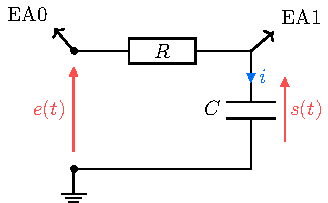
\includegraphics[width=.5\linewidth]{filtre_rc-sysam}
		\caption{Schéma complété.}
		\label{fig:rc-sysam}
	\end{figure}
}

\QR{%
	On souhaite éliminer toute composante continue des signaux observés,
	doit-on choisir le mode AC ou DC~? (vous pourrez faire une recherche sur
	internet ce que signifie mode AC et DC d'un oscilloscope).
}{%
	On choisit le mode \fbox{AC} (courant alternatif).
}


\QR{%
Si l'amplitude $E_{m}$ du signal d'entrée est représentée par
$\num{2,8}$ carreaux, en supposant que la sensibilité verticale est la
même sur les 2 voies, montrer que pour $f=f_{c}$ l'amplitude $S_{m}$ du
signal de sortie correspond alors à 2 carreaux sur l'oscillogramme.
}{%
À la fréquence coupure, on obtient
\[
	S_m(f_c) = \abs{\Hu(f_c)}E_m = \frac{E_m}{\sqrt{2}}
\]
L'application numérique donne bien $\xul{S_m(f_c) \approx \SI{2}{carreaux}}$.
}

\section{Réaliser}

\enonce{%
	\subsection{Étude rapide de comportement}

	\begin{tcb}(expe)<itc>{Diagramme automatique}
		\begin{enumerate}
			\item Connecter la carte Sysam à l'ordinateur~;
			\item Ouvrir \texttt{Oscillo5} (Programmes Physique-chimie $\rightarrow$
			      Eurosmart $\rightarrow$ \texttt{Oscillo5})~;
			\item Alimenter votre filtre RC avec la sortie analogique \texttt{SA1} de
			      la carte Sysam.
			\item Relever la tension $e(t)$ sur le canal \texttt{EA0} et la tension
			      $s(t)$ sur le canal \texttt{EA1}.
			\item Passer en mode \texttt{Bode}~;
			\item Afficher gain et phase~;
			\item Prendre une échelle log avec une étendue de fréquence cohérente avec
			      la fréquence de coupure que vous avez préalablement déterminée~;
			\item Sélectionner \texttt{EA0} en entrée~;
			\item Effacer acquisitions précédentes. Choisir~: toutes~;
			\item Déclencher.
			\item Les diagrammes sont tracés de manière automatique. Pratique si on
			      veut être rapide~!
		\end{enumerate}
	\end{tcb}
}

\setcounter{subsection}{1}
\subsection{Mesures pour le tracé du diagramme de \textsc{Bode}}

\enonce{%
	Il s'agit maintenant de faire un relevé fréquence par fréquence pour apprendre
	à le faire «~à la main~».

	\begin{tcb}(expe)<itc>{À la main}
		\begin{enumerate}
      \item Choisir maintenant le mode \texttt{BALAYAGE}, pour utiliser
            \texttt{Oscillo5} comme un oscilloscope~;
      \item Dans le panneau de contrôle (boîte flottante en haut de l'écran),
            cliquer sur \texttt{Voir GBF1} et appuyer sur \texttt{Marche}~;
      \item Prendre comme amplitude du signal d'entrée environ $\SI{2}{V}$ (soit
            $\SI{4}{Vpp}$). Pour des fréquences entre \SI{100}{Hz} et
            \SI{50}{kHz}~:
			\item Mesurer le déphasage entre $s(t)$ et $e(t)$ à l'aide d'Oscillo5,
			      comme indiqué dans S'approprier. Pour plus de facilité, utiliser
            les curseurs (en bas à droite du menu d'Oscillo5) et les calibres
            horizontaux (à droite) et verticaux (en bas).
			\item Mesurer le gain en dB à l'aide du dBmètre, comme indiqué dans
			      S'approprier.
			\item Une échelle logarithmique de variation de la fréquence est
			      pertinente et vous pourrez faire plus de mesures autour de la
			      fréquence de coupure $f_{c}$ précédemment établie.
		\end{enumerate}
	\end{tcb}
}

\resetQ
\setlist[blocQR,1]{leftmargin=10pt, label=\sqenumi}
\QR{%
	Regrouper les valeurs dans un tableau~:
	\begin{table}[htbp!]
		\centering
		\caption{Mesures pour diagramme de \textsc{Bode}.}
		\begin{tabularx}{\linewidth}{YYYYY}
			\toprule
			$f$ (\si{Hz})                       &
			$G\ind{dB}$ (\si{dB})               &
			$\abs{\Delta{t}}$ (\si{s})          &
			$\abs{\Delta{\f_{s/e}}}$ (\si{rad}) &
			$\Delta{\f_{s/e}}$ (rad)
			\\
			\midrule
			$\vdots$                            &
			$\vdots$                            &
			$\vdots$                            &
			$\vdots$                            &
			$\vdots$
			\\
			$\vdots$                            &
			$\vdots$                            &
			$\vdots$                            &
			$\vdots$                            &
			$\vdots$
			\\
			\bottomrule
		\end{tabularx}
		\label{tab:ddb}
	\end{table}
}{%
	\begin{table}[htbp!]
		\centering
		\caption{Mesures pour diagramme de \textsc{Bode}.}
		\begin{tabularx}{\linewidth}{YYYYY}
			\toprule
			$f$ (\si{Hz})                             &
			$G\ind{dB}$ (\si{dB})                     &
			$\abs{\Delta{t}}$ (\si{s})                &
			$\abs{\Delta{\f_{s/e}}}$ (\si{rad})       &
			$\Delta{\f_{s/e}}$ (rad)
			\\
			\midrule
			$\py{fr'\num{{{flist[0]}}}'}$         &
			$\py{fr'\num{{{G(flist[0]):.2f}}}'}$      &
			$\py{fr'\num{{{T(flist[0]):.2e}}}'}$      &
			$\py{fr'\num{{{abs(F(flist[0])):.2f}}}'}$ &
			$\py{fr'\num{{{F(flist[0]):.2f}}}'}$
			\\
			$\py{fr'\num{{{flist[1]}}}'}$         &
			$\py{fr'\num{{{G(flist[1]):.2f}}}'}$      &
			$\py{fr'\num{{{T(flist[1]):.2e}}}'}$      &
			$\py{fr'\num{{{abs(F(flist[1])):.2f}}}'}$ &
			$\py{fr'\num{{{F(flist[1]):.2f}}}'}$
			\\
			$\py{fr'\num{{{flist[2]}}}'}$         &
			$\py{fr'\num{{{G(flist[2]):.2f}}}'}$      &
			$\py{fr'\num{{{T(flist[2]):.2e}}}'}$      &
			$\py{fr'\num{{{abs(F(flist[2])):.2f}}}'}$ &
			$\py{fr'\num{{{F(flist[2]):.2f}}}'}$
			\\
			$\py{fr'\num{{{flist[3]}}}'}$         &
			$\py{fr'\num{{{G(flist[3]):.2f}}}'}$      &
			$\py{fr'\num{{{T(flist[3]):.2e}}}'}$      &
			$\py{fr'\num{{{abs(F(flist[3])):.2f}}}'}$ &
			$\py{fr'\num{{{F(flist[3]):.2f}}}'}$
			\\
			$\py{fr'\num{{{flist[4]}}}'}$         &
			$\py{fr'\num{{{G(flist[4]):.2f}}}'}$      &
			$\py{fr'\num{{{T(flist[4]):.2e}}}'}$      &
			$\py{fr'\num{{{abs(F(flist[4])):.2f}}}'}$ &
			$\py{fr'\num{{{F(flist[4]):.2f}}}'}$
			\\
			$\py{fr'\num{{{flist[5]}}}'}$         &
			$\py{fr'\num{{{G(flist[5]):.2f}}}'}$      &
			$\py{fr'\num{{{T(flist[5]):.2e}}}'}$      &
			$\py{fr'\num{{{abs(F(flist[5])):.2f}}}'}$ &
			$\py{fr'\num{{{F(flist[5]):.2f}}}'}$
			\\
			$\py{fr'\num{{{flist[6]}}}'}$         &
			$\py{fr'\num{{{G(flist[6]):.2f}}}'}$      &
			$\py{fr'\num{{{T(flist[6]):.2e}}}'}$      &
			$\py{fr'\num{{{abs(F(flist[6])):.2f}}}'}$ &
			$\py{fr'\num{{{F(flist[6]):.2f}}}'}$
			\\
			$\py{fr'\num{{{flist[7]}}}'}$         &
			$\py{fr'\num{{{G(flist[7]):.2f}}}'}$      &
			$\py{fr'\num{{{T(flist[7]):.2e}}}'}$      &
			$\py{fr'\num{{{abs(F(flist[7])):.2f}}}'}$ &
			$\py{fr'\num{{{F(flist[7]):.2f}}}'}$
			\\
			$\py{fr'\num{{{flist[8]}}}'}$         &
			$\py{fr'\num{{{G(flist[8]):.2f}}}'}$      &
			$\py{fr'\num{{{T(flist[8]):.2e}}}'}$      &
			$\py{fr'\num{{{abs(F(flist[8])):.2f}}}'}$ &
			$\py{fr'\num{{{F(flist[8]):.2f}}}'}$
			\\
			$\py{fr'\num{{{flist[9]}}}'}$         &
			$\py{fr'\num{{{G(flist[9]):.2f}}}'}$      &
			$\py{fr'\num{{{T(flist[9]):.2e}}}'}$      &
			$\py{fr'\num{{{abs(F(flist[9])):.2f}}}'}$ &
			$\py{fr'\num{{{F(flist[9]):.2f}}}'}$
			\\
			$\py{fr'\num{{{flist[10]}}}'}$         &
			$\py{fr'\num{{{G(flist[10]):.2f}}}'}$      &
			$\py{fr'\num{{{T(flist[10]):.2e}}}'}$      &
			$\py{fr'\num{{{abs(F(flist[10])):.2f}}}'}$ &
			$\py{fr'\num{{{F(flist[10]):.2f}}}'}$
			\\
			$\py{fr'\num{{{flist[11]}}}'}$         &
			$\py{fr'\num{{{G(flist[11]):.2f}}}'}$      &
			$\py{fr'\num{{{T(flist[11]):.2e}}}'}$      &
			$\py{fr'\num{{{abs(F(flist[11])):.2f}}}'}$ &
			$\py{fr'\num{{{F(flist[11]):.2f}}}'}$
			\\
			$\py{fr'\num{{{flist[12]}}}'}$         &
			$\py{fr'\num{{{G(flist[12]):.2f}}}'}$      &
			$\py{fr'\num{{{T(flist[12]):.2e}}}'}$      &
			$\py{fr'\num{{{abs(F(flist[12])):.2f}}}'}$ &
			$\py{fr'\num{{{F(flist[12]):.2f}}}'}$
			\\
			$\py{fr'\num{{{flist[13]}}}'}$         &
			$\py{fr'\num{{{G(flist[13]):.2f}}}'}$      &
			$\py{fr'\num{{{T(flist[13]):.2e}}}'}$      &
			$\py{fr'\num{{{abs(F(flist[13])):.2f}}}'}$ &
			$\py{fr'\num{{{F(flist[13]):.2f}}}'}$
			\\
			$\py{fr'\num{{{flist[14]}}}'}$         &
			$\py{fr'\num{{{G(flist[14]):.2f}}}'}$      &
			$\py{fr'\num{{{T(flist[14]):.2e}}}'}$      &
			$\py{fr'\num{{{abs(F(flist[14])):.2f}}}'}$ &
			$\py{fr'\num{{{F(flist[14]):.2f}}}'}$
			\\
			\bottomrule
		\end{tabularx}
		\label{tab:ddb_corr}
	\end{table}

% 	\begin{table}[htbp!]
% 		\centering
% 		\caption{TESTTEST}
% \begin{pycode}
% print(r"\begin{tabularx}{\linewidth}{YYYYY}")
% print(r"\toprule")
% print(r"$f$ (\si{Hz})                             &")
% print(r"$G\ind{dB}$ (\si{dB})                     &")
% print(r"$\abs{\Delta{t}}$ (\si{s})                &")
% print(r"$\abs{\Delta{\f_{s/e}}}$ (\si{rad})       &")
% print(r"$\Delta{\f_{s/e}}$ (rad)")
% print(r"\\"
% print(r"\midrule")
% for n in range(0,15):
%     print(fr'\num{{{flist[{n}]}}} & \num{{{G(flist[{n}]):.2f}}} & \num{{{T(flist[{n}]):.2e}}} & \num{{{abs(F(flist[{n}])):.2f}}} & \num{{{F(flist[{n}]):.2f}}}\\')
% print(r"\bottomrule")
% print(r"\end{tabularx}")
% \end{pycode}
% 	\end{table}
}

\section{Valider et conclure}

\QR{%
	Tracer le diagramme de \textsc{Bode} expérimental sur papier semi-log
	(fourni en fin de sujet) en mettant la fréquence en abscisse (les 2 courbes
	sur une même feuille en prenant l'échelle du gain en haut et l'échelle du
	déphasage en bas).
}{%
	Voir fin du sujet.
}

\QR{%
	Ajouter sur le diagramme, les asymptotes obtenues grâce à l'étude
	théorique de l'analyse.
}{%
	Idem.
}
\begin{blocQR}{}
	\item En déduire~:
	\QR{%
		La fréquence de coupure expérimentale $f_{c, \exp}$ en considérant
		$G_{\dB}(f_{c, \exp}) = G_{\dB, max} -\SI{3}{dB}$. La comparer à la valeur
		théorique en calculant l'écart \textbf{normalisé}.
	}{%
		On trouve $f_{c, \exp} = \SI{1.57\pm0.02}{kHz}$, d'où l'écart normalisé
    \[
      \boxed{E_n = \frac{\abs{f_{c, \exp} - f_{c, \rm theo}}}{u_{f_{c, \exp}}}}
      \Ra 
      \xul{E_n = 1} < 2
      \quad \text{donc compatibles.}
    \]
	}

	\QR{%
	Le déphasage expérimental $\f_{c, \exp}$ pour $f=f_{c, \exp}$. Le comparer à
	la valeur théorique en calculant l'écart \textbf{normalisé}.
	}{%
	 Calcul similaire.
	}

	\QR{%
		La nature du filtre.
	}{%
		C'est un passe-bas.
	}

\end{blocQR}

\newpage

\thispagestyle{empty}
\cswitch{
  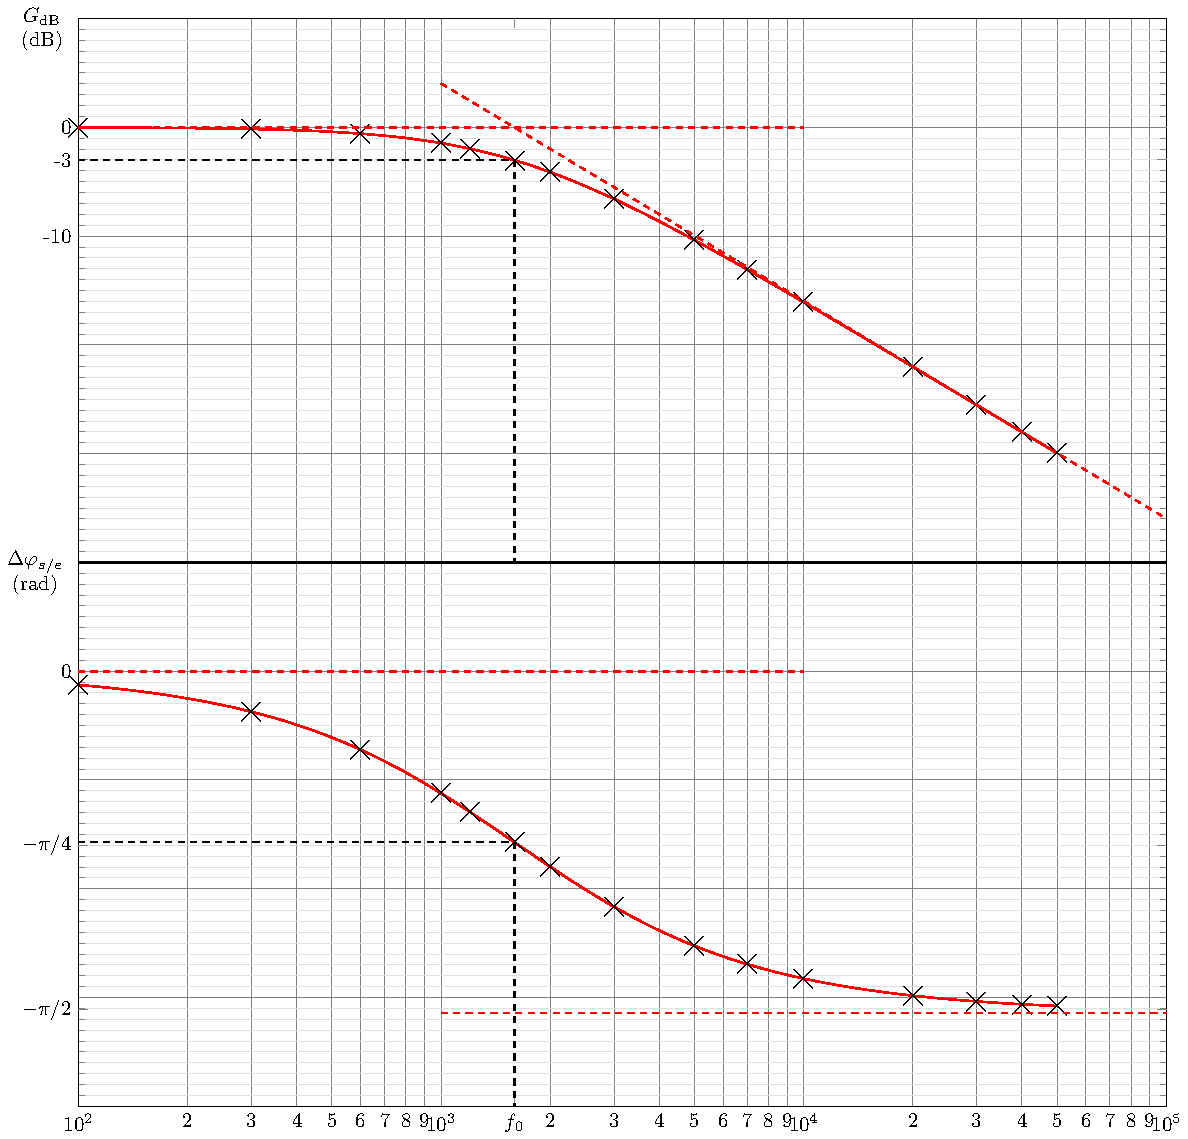
\includepdf{semilog_solu}
}{
  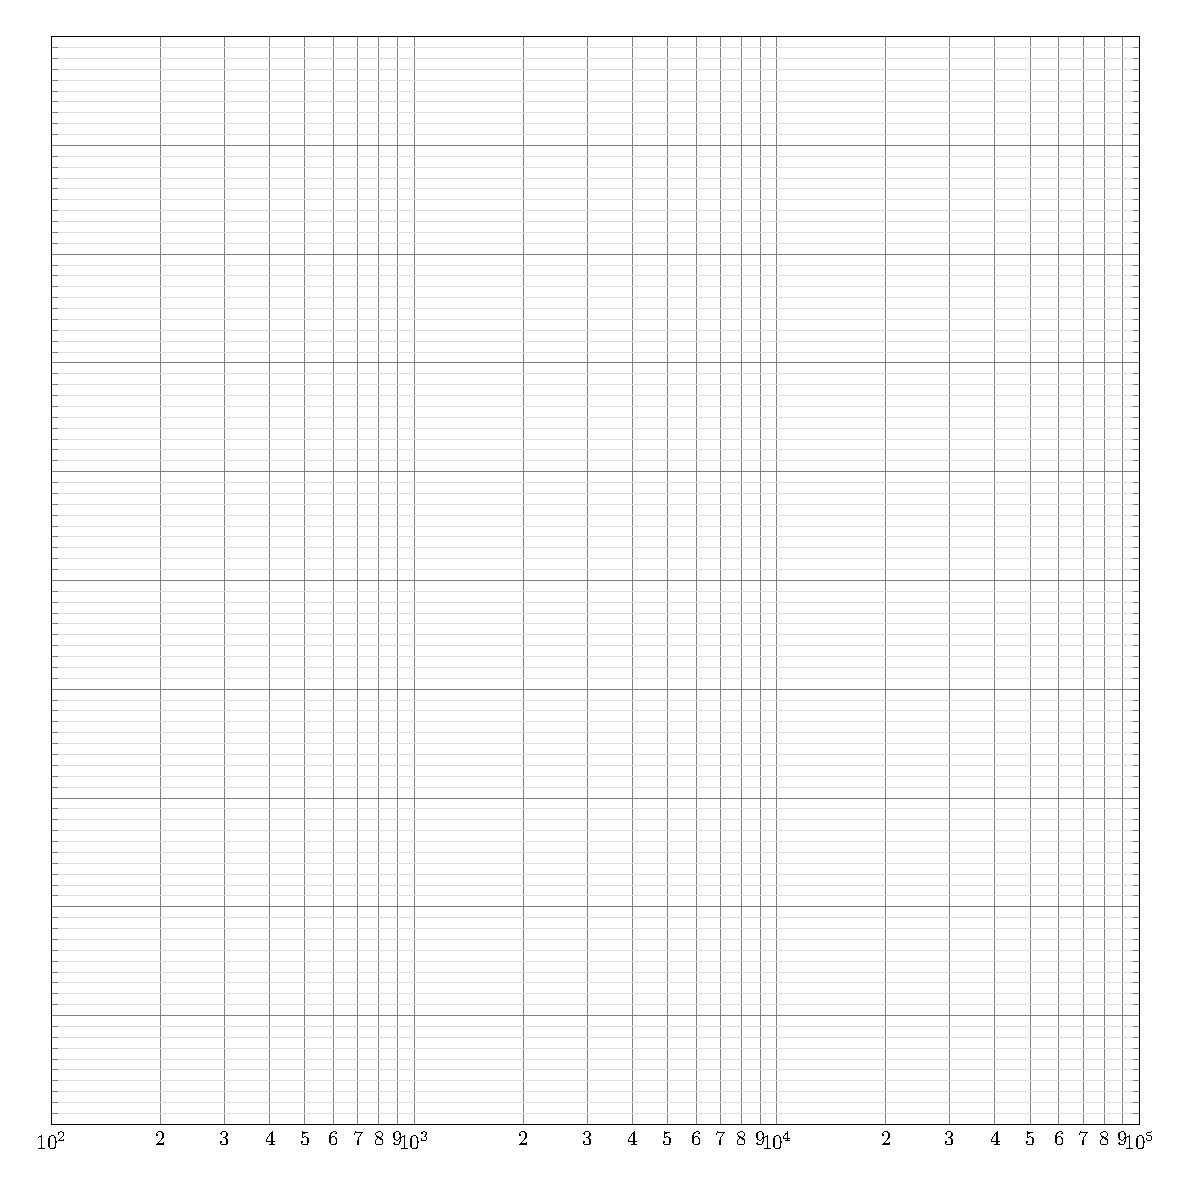
\includepdf{semilog}
}

\let\clearpage\relax

\end{document}
